\section{Przebieg ćwiczenia}
\subsection{Modyfikacja projektu z laboratorium 3}
Skopiowano folder lab3 do nowego folderu lab4, a następnie otwarto go w programie XPS.

\subsection{Dodanie BRAM i kontroler BRAM}
Z katalogu IP dodano następujące IP do projektu systemu:
\begin{itemize}
	\item XPS BRAM Controller 1.00.b
	\item Block RAM (BRAM) block 1.00.a
\end{itemize}

Następnie połączono kontroler BRAM do PLB i BRAM do kontrolera BRAM.

\begin{figure}[h]
	\centering
	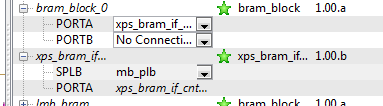
\includegraphics{img/add_ram.PNG}
	\label{img:add_ram}
	\caption{Dodane i połączone IP BRAM i BRAM controller}
\end{figure}

W zakładce "Adresses" ustawiono rozmiar pamięci BRAM na 8K i kliknięto na przycisk "Generate Adresses"

W menu "Hardware" kliknięto na "Generate Bitstream". Później w menu "Project" kliknięto "Export Hardware Design to SDK" a następnie "Export \& Launch SDK".

\newpage
\subsection{Tworzenie aplikacji}
Po otworzeniu SDK w odpowiednim folderze, utworzono nowy projekt typu "Xilinx C Project". Wybrano szablon "Empty Application" a jako nazwę podano "TestApp". Następnie wybrano odpowiedni BSP. Zaimportowano plik lab4.c.

\begin{figure}[h]
	\centering
	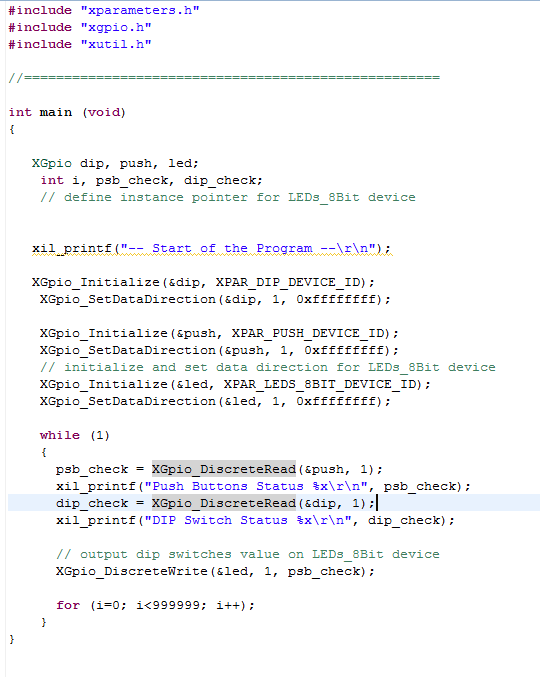
\includegraphics{img/program_1.PNG}
	\label{img:program_1}
	\caption{Zaimporowany program}
\end{figure}

Po przeczytaniu dokumentacji zmodyfikowano kod tak, aby na diodach LED wyświetlany był stan przycisków i przełączników.

\lstinputlisting[language=C]{zmodyfikowany.c}

\subsection{Analiza zbudowanych obiektów}
W menu "Xilinx Tools" kliknięto na "Generate Linker Script". Następnie zmieniono rozmiar stosu i stogu na 400 bajtów i kliknięto "Generate".

Zrekompilowano plik lab4.c, a następnie w menu "Xilinx Tools" wybrano "Launch shell". Komenda \verb+cd+ została użyta aby przejść do folderu \verb+TestApp/Debug+.

Użyto komendy \verb`mb-objdump -h TestApp.elf` do wyświetlenia poszczególnych sekcji programu.
\newpage


\begin{figure}[h]
	\centering
	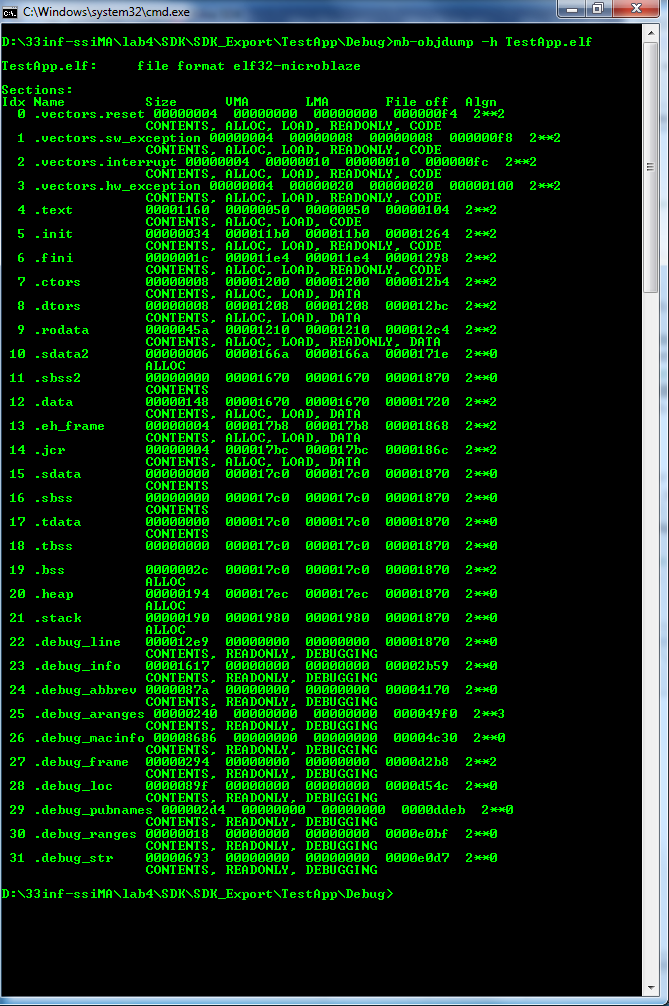
\includegraphics[height=20cm]{img/objdump.PNG}
	\label{img:objdump}
\end{figure}

Ponownie otwarto okno "Generate Linker Script". Rozmiary stosu i stogu zostały zmienione na 1KB. Następnie w liście rozwijanej "Place Code Sections in: " wybrano kontroler BRAM.
\newpage
Po ponownej rekompilacji pliku lab4.c i uruchomieniu komendy \verb+mb-objdump+ zauważono, że sekcja .text przesunęła się do pamięci BRAM.

\subsection{Weryfikacja w sprzęcie}
Używając narzędzia "Program FPGA" wgrano aplikację na płytkę i zweryfikowano, że działa

\begin{figure}[h]
	\centering
	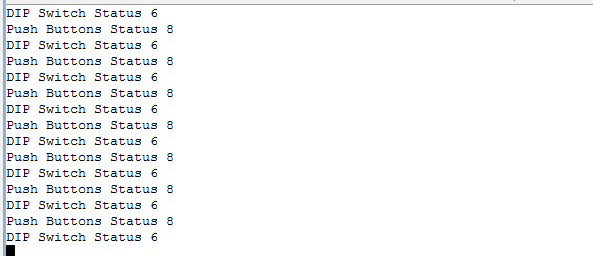
\includegraphics{img/putty-dziala.PNG}
	\label{img:putty-dziala}
\end{figure}
